\chapter{Our Work}
\label{ch:ourwork}

\section{Motivation}
The forecasting finance area is currently under intense research focus: many researchers
and specialists are trying to combine Time2Vec with CNN, RNN, LSTM, and
Attention mechanism. Moreover, not only finance but also other fields as well
like Aeroengine Risk Assessment \cite{10278395} and Predicting Production in
Shale and Sandstone Gas Reservoirs \cite{FARGALLA2024130184}.

They usually use only one feature to predict things (for instance, only one
stock price to predict its prices). However, using techniques that rely solely on
a single feature can be quite challenging when it comes to predicting unexpected
financial events, which are often influenced by external factors beyond our
control. On the flip side, in the world of finance, it's common practice to focus
on identifying and analyzing correlations between specific features and target prices
when making investment decisions.

Building upon previous challenges, we were motivated to explore the integration
of correlations from multiple features into the Transformer model. We represents
a new approaches over existing methods by developing a neural network architecture
that consists of Time2Vec, residual, multiple attention layers, pooling, and a dense
fully-connected part. Given the limitations inherent in financial data often
sparse and messy we sought to address these issues by selecting multiple stocks
exhibiting similar behavior and interconnectedness. The subsequent sections of this
paper will detail our approach to time series modeling.

\section{Methodology}
The performance of a stock market predictor heavily depends on the correlations between
historical data for training and the current input for prediction. The results
show below here in \autoref{fig:exx_base} and \autoref{fig:nas_base} we use
Exxon Mobil and NASDAQ stock prices as base market.

\begin{figure}[H]
	\centering
	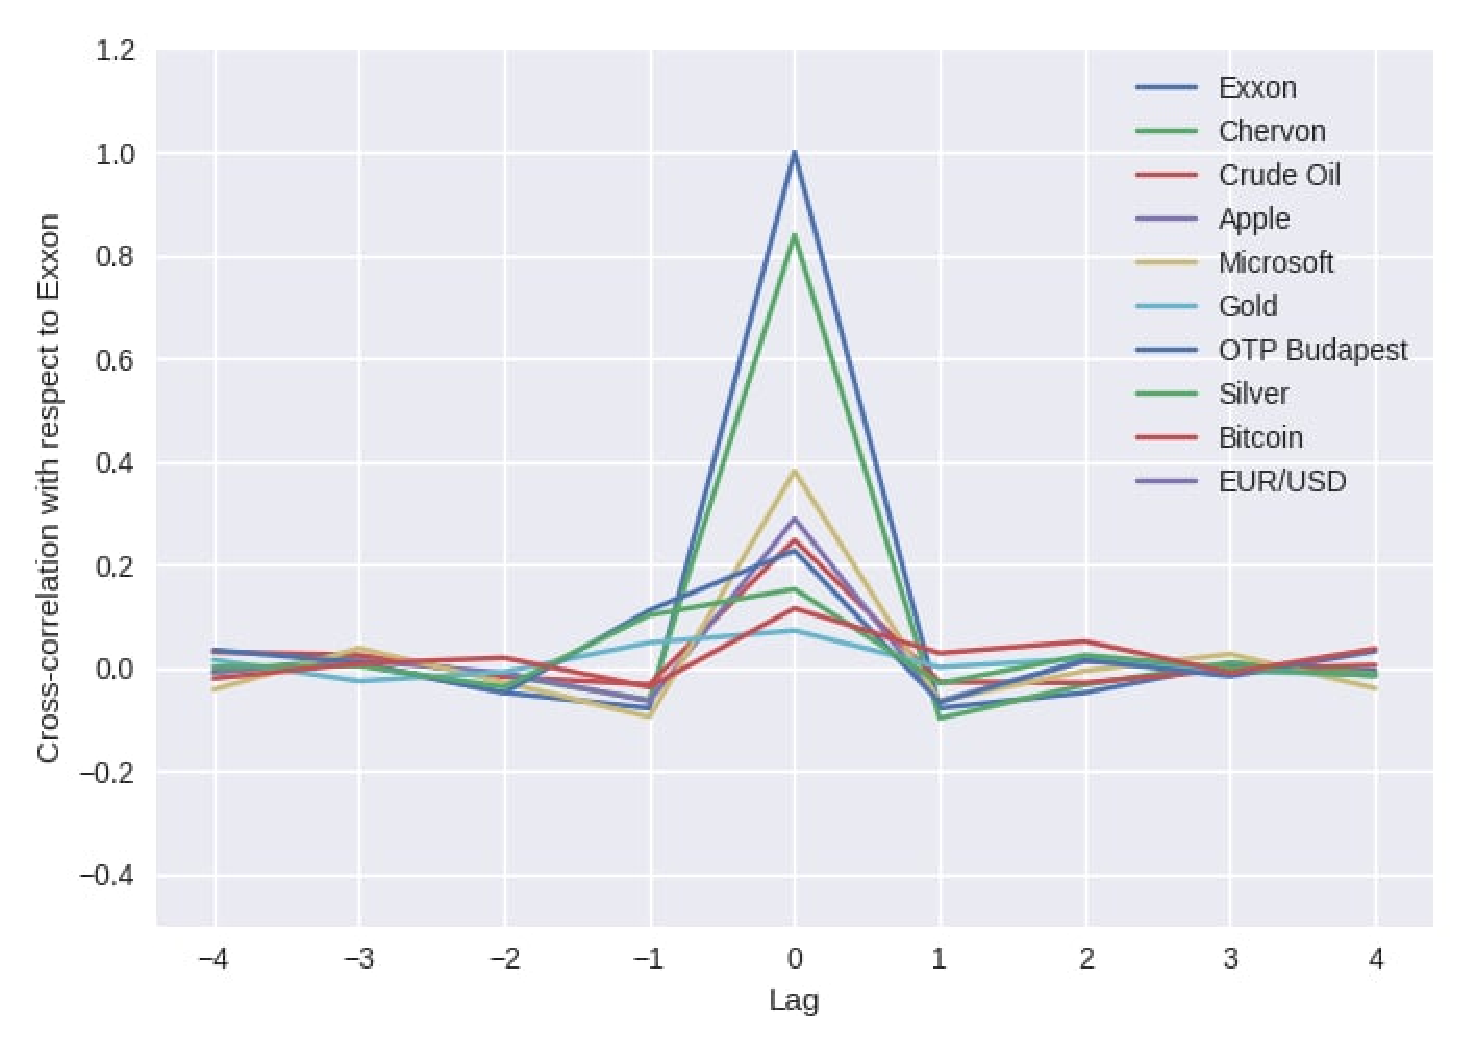
\includegraphics[width=1\linewidth]{images/exx_base.eps}
	\caption{Auto-correlation and cross-correlation of markets trend using Exxon
		Mobil as a based market.}
	\label{fig:exx_base}
\end{figure}

The graph (\autoref{fig:exx_base}) reveals that base markets' auto-correlation is solely non-zero at the origin.
This observation suggests that the daily trend of Exxon stock approximates a
Markov process \cite{Shen2012StockMF}. Consequently, historical data offers
limited insight into its future movements. However, data source such as Chevron
is a promising feature for our approach.

\begin{figure}[H]
	\centering
	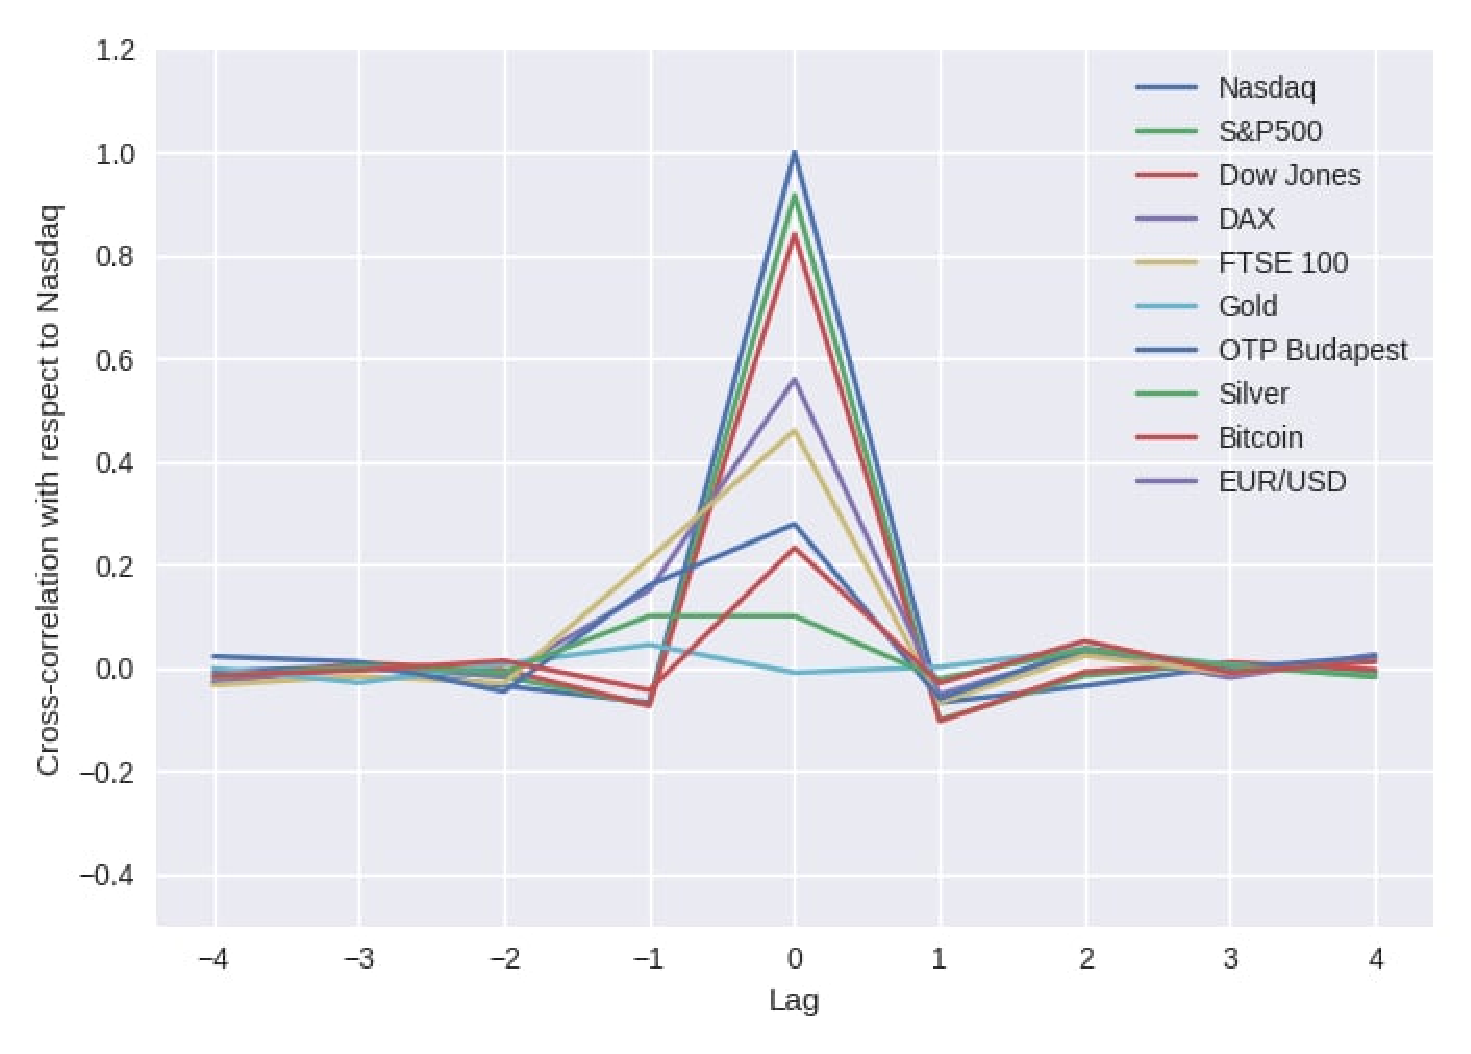
\includegraphics[width=1\linewidth]{images/nas_base.eps}
	\caption{Auto-correlation and cross-correlation of markets trend using NASDAQ
		as a based market.}
	\label{fig:nas_base}
\end{figure}

From \autoref{fig:nas_base} we get same conclusion for NASDAQ, S\&P500 will be a good data to pair with. Moreover, we will try to evaluate will it be better if we put more relatable data (for example: NASDAQ, S\&P500, Dow Jones, and DAX into the model) than only 2 features (NASDAQ and S\&P500).

\section{Mean Not NaN}
Each time series might have missing data points represented as NaN values, and we have to use a proper combination approach that handles this issue. In this paper, we considered Geometry Mean Not NaN - GMNN (\autoref{fig:gmnn}) and Arithmetic Mean Not NaN - AMNN (\autoref{fig:amnn}).

\subsection{Geometry Mean Not NaN - GMNN}
GMNN is the technique we find out to combine multiple normalized data into one
normalized data. This technique assure that the transformed data will be between
0 and 1 – which is the attribute the combined data must have.

\begin{figure}[H]
	\centering
	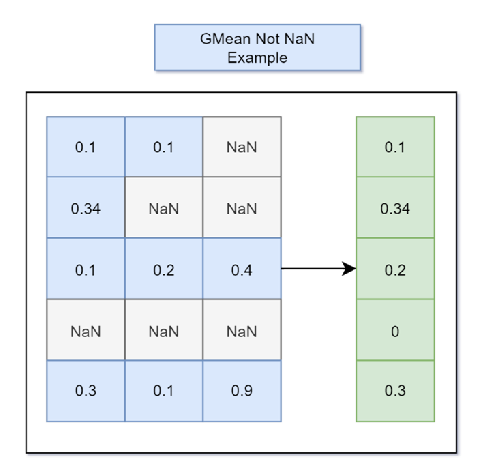
\includegraphics[width=0.7\linewidth]{images/gmnn.eps}
	\caption{Simple illustration with 1-Dimensional input pass through GMNN step.}
	\label{fig:gmnn}
\end{figure}

How do GMNN work? – GMNN iterate by row and take the Geometry Mean of real numbers
in each row and assign it as a output value for that row.

\subsection{Arithmetic Mean Not NaN - AMNN}
AMNN follows the same idea with GMNN that is combining multiple normalized data into
one normalized data.

AMNN iterate by row and take the Arithmetic Mean of real numbers in each row and
assign it as a output value for that row.

\begin{figure}[H]
	\centering
	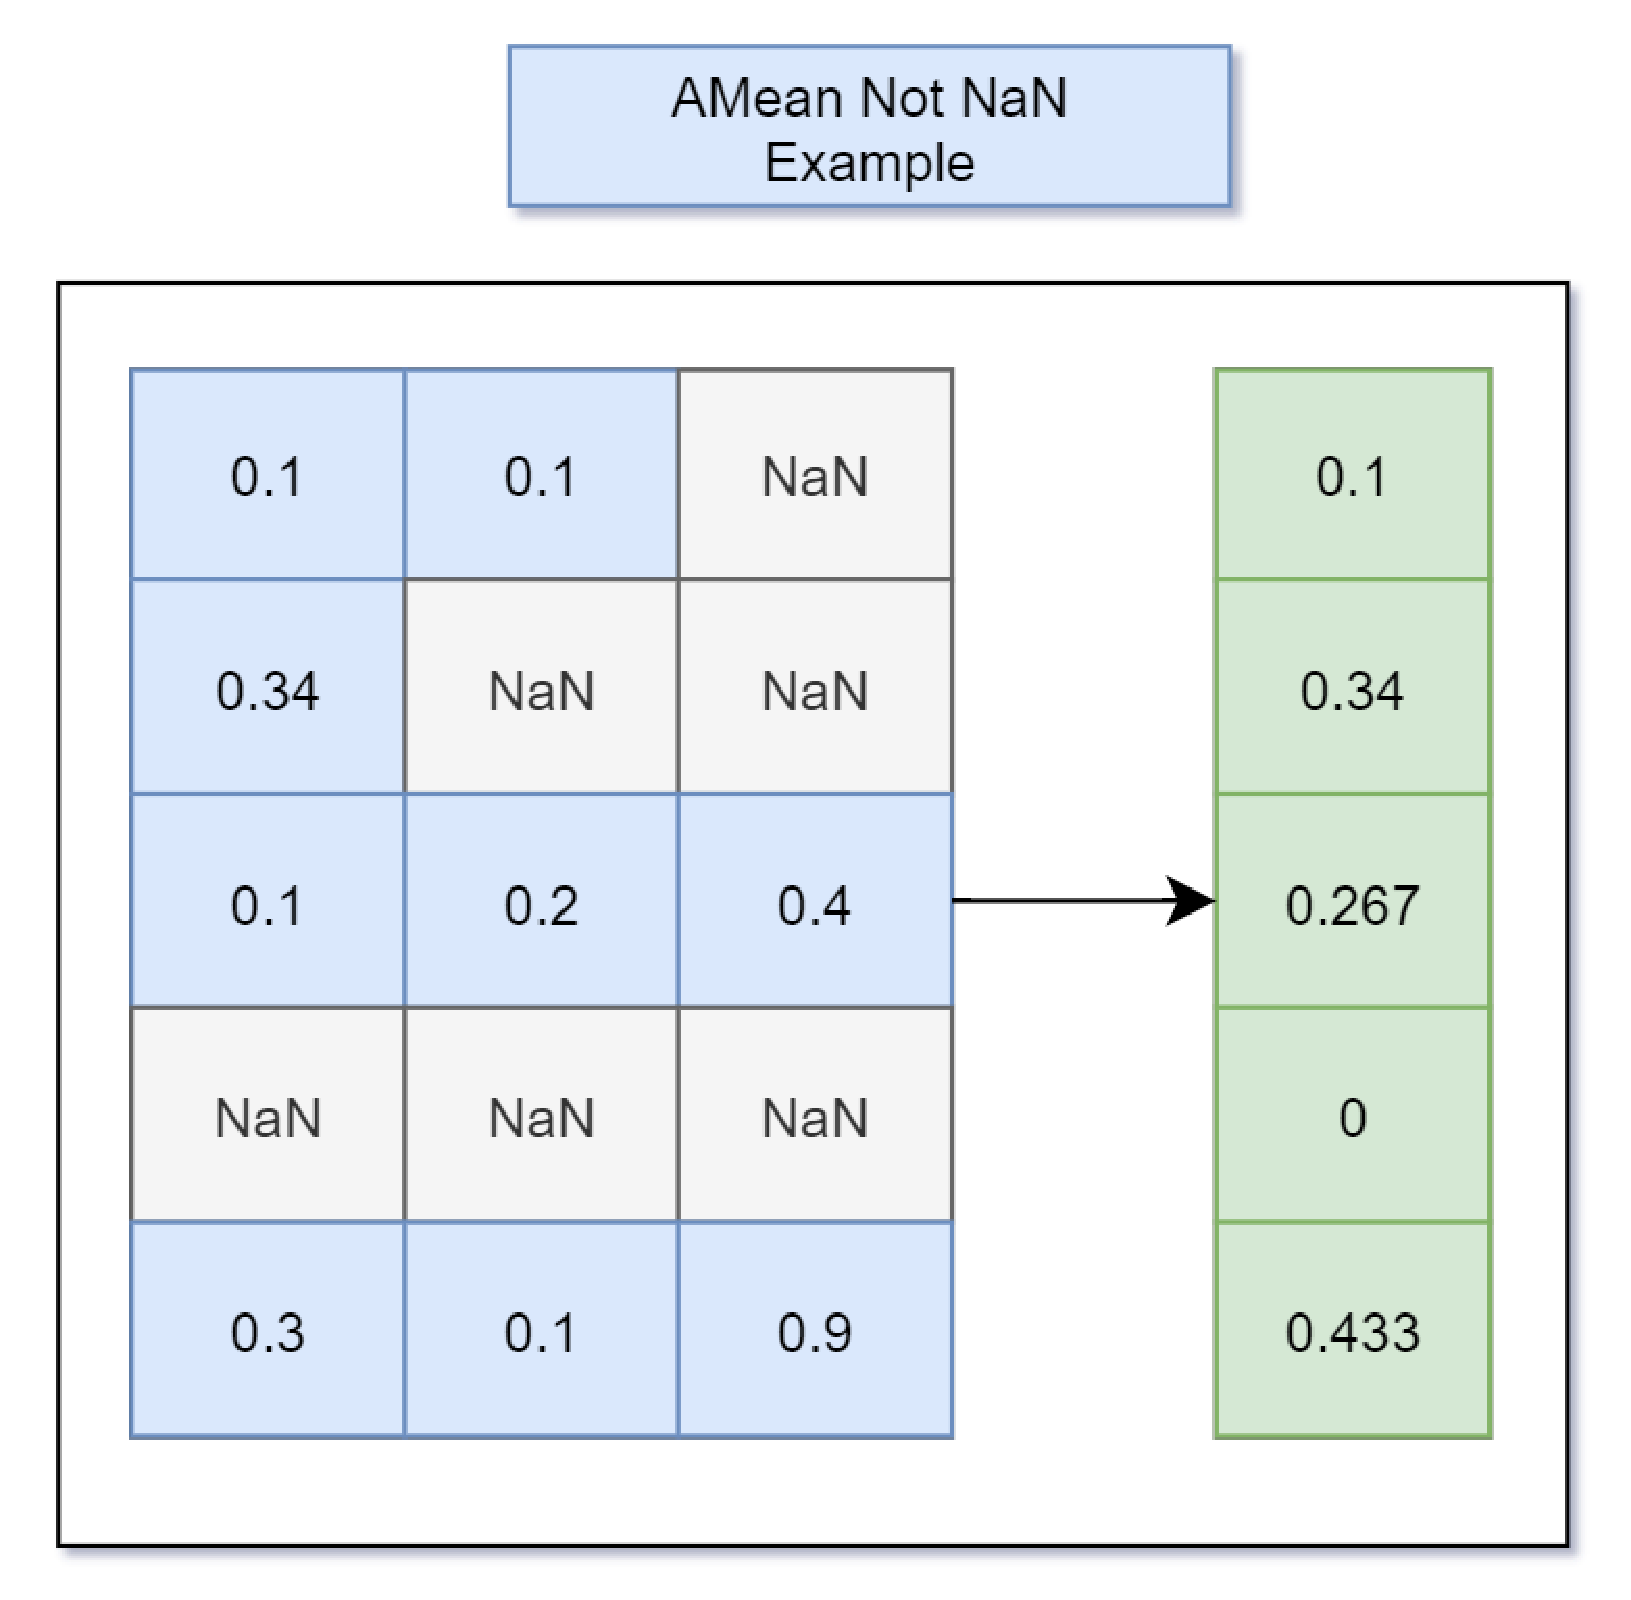
\includegraphics[width=0.7\linewidth]{images/amnn.eps}
	\caption{Simple illustration with 1-Dimensional input pass through AMNN step.}
	\label{fig:amnn}
\end{figure}

\subsection{AMNN or GMNN?}
Both AMNN and GMNN can resolve the task. However, by experiment several times, we
can conclude that GMNN yields better result in predicting stock prices than AMNN,
so that we will choose GMNN as a method to represent our result in this thesis.